\documentclass{standalone}
\usepackage{tikz}
\usetikzlibrary{calc,patterns,decorations.pathmorphing,decorations.markings}

\begin{document}

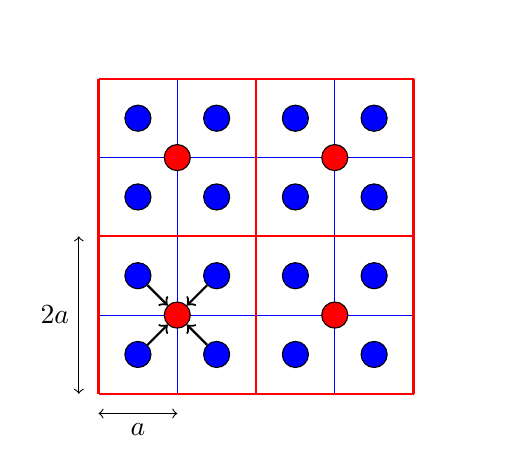
\begin{tikzpicture}

\draw[step=1cm,blue, thin] (0,0) grid (4,4);
\draw[step=2cm,red, thick] (0,0) grid (4,4);

\foreach \i in {0, ..., 3}
{
	\foreach \j in {0, ..., 3}
	{
		\node[circle,fill=blue,draw=black,radius=2pt](fine\i \j) at ($+\i*(1,0)+\j*(0,1)+(.5,.5)$){};
	}
}

\foreach \i in {0,2, ..., 2}
{
	\foreach \j in {0,2, ..., 2}
	{
		\node[circle,fill=red,draw=black,radius=4pt](coarse\i \j) at ($\i*(1,0)+\j*(0,1)+(1,1)$){};								
	}
}

%draw aligned value
\draw[->,thick](fine00)--(coarse00);
\draw[->,thick](fine10)--(coarse00);
\draw[->,thick](fine01)--(coarse00);
\draw[->,thick](fine11)--(coarse00);

%add annotations
\draw[<->](0,-.25)--node[below]{$a$}(1,-.25);
\draw[<->](-.25,0)--node[left]{$2a$}(-.25,2);
\draw[draw=none](-.9,-.65) rectangle (4.9,4.65);
\end{tikzpicture}

\end{document}